\documentclass{article}

%other packages
\usepackage[a4paper, total={7.5in, 10.5in}]{geometry}
\usepackage{longtable}
\usepackage{wrapfig}
\setlength\parindent{0pt}
\usepackage{enumitem}
\usepackage[table]{xcolor}
\usepackage{polynom}
\usepackage{nopageno}

%maths
\usepackage{mathtools}
\usepackage{amsmath}
\usepackage{amssymb}
\usepackage{amsfonts}
\usepackage{autobreak}

%tikzpicture
\usepackage{tikz}
\usepackage{scalerel}
\usepackage{pict2e}
\usepackage{tkz-euclide,comment}
\usetikzlibrary{calc}
\usetikzlibrary{patterns,arrows.meta}
\usetikzlibrary{shadows}
\usetikzlibrary{external}

%pgfplots
\usepackage{pgfplots}
\pgfplotsset{compat=newest}
\usepgfplotslibrary{statistics}
\usepgfplotslibrary{fillbetween}
\usepgfplotslibrary{polar}

\pgfplotsset{
    standard/.style={
    axis line style = thick,
    trig format=rad,
    axis equal,
    enlargelimits,
    axis x line=middle,
    axis y line=middle,
    enlarge x limits=0.15,
    enlarge y limits=0.15,
    every axis x label/.style={at={(current axis.right of origin)},anchor=north west},
    every axis y label/.style={at={(current axis.above origin)},anchor=south east}
    }
}
\begin{document}


\centering

Prove the formula $a=\frac{1}{2}r^2\theta$ for the area of a sector of a circle with radius $r$ and central angle $\theta$. [\textit{Hint:} Assume $0<\theta<\pi/2$ and place the center of the circle at the origin so it has equation $x^2+y^2=r^2$. Then $A$ is the sum of the area of the triangle $POQ$ and the area of the region $PQR$ in the figure.]

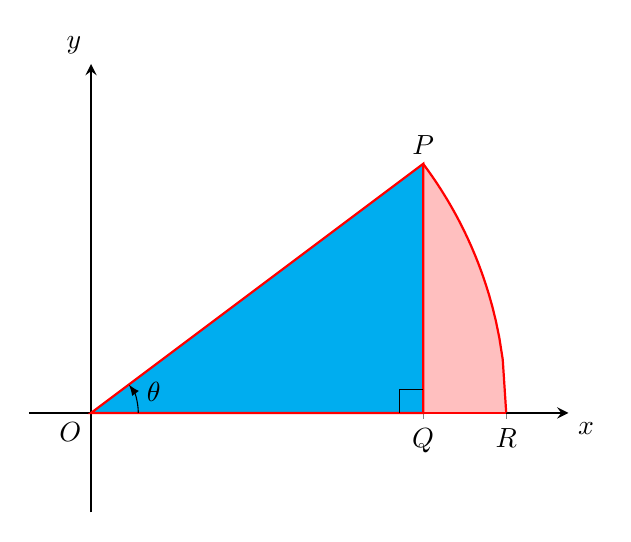
\begin{tikzpicture}
\begin{axis}[standard,xmin=0,trig format=deg,xtick={0.8,1},xticklabels={$Q$,$R$},ytick={\empty},xlabel={$x$},ylabel={$y$}]
\addplot[domain=0.8:1,red,thick,name path=F]{(1-x^2)^(1/2)};
\coordinate (A) at (0,0);
\coordinate (B) at (0.8,0.6);
\coordinate (C) at (0.8,0);
\draw[red,thick,fill=cyan] (A) -- (B) -- (C) -- cycle;
\draw pic["$\theta$",draw,-latex,angle eccentricity=1.4, angle radius=0.6cm]{angle=C--A--B};
\draw pic[draw,-,angle eccentricity=1.4, angle radius=0.3cm]{right angle=B--C--A};
\node[anchor=north east] at (0,0) {$O$};
\node[anchor=south] at (0.8,0.6) {$P$};
\draw[red,thick,name path=G] (0.8,0) -- (1,0);
\addplot[fill=pink] fill between [of=F and G, soft clip={domain=0.8:1}];
\end{axis}
\end{tikzpicture}

\[A=\frac{r^2}{2}\sin\theta\cos\theta+\int_{r\cos\theta}^r\sqrt{r^2-x^2}\ dx\]
\[\mbox{let }x=r\cos\theta,\ dx=-r\sin\theta\ d\theta\]

\begin{tikzpicture}[scale=7]
\coordinate (A) at (0,0);
\coordinate (B) at (30:1);
\coordinate (C) at (30:1|-0,0);
\draw (A) -- node[pos=0.5,above left]{$r$} (B) -- node[pos=0.5,right]{$\sqrt{r^2-x^2}$} (C) -- node[pos=0.5,below]{$x$} (A);
\draw pic["$\theta$",draw,-,angle eccentricity=1.4, angle radius=0.6cm]{angle=C--A--B};
\draw pic[draw,-,angle eccentricity=1.4, angle radius=0.3cm]{right angle=B--C--A};
\end{tikzpicture}

Now we will solve the indefinite integral $\int\sqrt{r^2-x^2}\ dx$.

\begin{align*}
\int\sqrt{r^2-x^2}\ dx&\overset{x=r\cos\theta}{\underset{dx=-r\sin\theta\ d\theta}{=\joinrel=\joinrel=\joinrel=\joinrel=\joinrel=\joinrel=\joinrel=}}-r^2\int\sin^2\theta\ d\theta\\
&=-\frac{r^2}{2}\int1-\cos2\theta\ d\theta\\
&=-\frac{r^2}{2}[\theta-\frac{1}{2}\sin2\theta]+C\\
&=-\frac{r^2}{2}[\theta-\sin\theta\cos\theta]+C\\
&=-\frac{r^2}{2}[\theta-\frac{\sqrt{r^2-x^2}}{r}\cdot\frac{x}{r}]+C\\
&=-\frac{r^2}{2}\arccos\frac{x}{r}+\frac{x}{2}\sqrt{r^2-x^2}+C
\end{align*}

Now we will apply the original boundaries.

\begin{align*}
\int_{r\cos\theta}^r\sqrt{r^2-x^2}\ dx&=\left[-\frac{r^2}{2}\arccos\frac{x}{r}+\frac{x}{2}\sqrt{r^2-x^2}\right]_{r\cos\theta}^r\\
&=\frac{r^2}{2}\theta-\frac{r^2}{2}\sin\theta\cos\theta
\end{align*}

Solving, we get:

\[\frac{r^2}{2}\sin\theta\cos\theta+\int_{r\cos\theta}^r\sqrt{r^2-x^2}\ dx=\frac{r^2}{2}\sin\theta\cos\theta+\frac{r^2}{2}\theta-\frac{r^2}{2}\sin\theta\cos\theta=\frac{r^2}{2}\theta\]

\newpage



\centering







Prove the formula $a=\frac{1}{2}r^2\theta$ for the area of a sector of a circle with radius $r$ and central angle $\theta$. [\textit{Hint:} Assume $0<\theta<\pi/2$ and place the center of the circle at the origin so it has equation $x^2+y^2=r^2$. Then $A$ is the sum of the area of the triangle $POQ$ and the area of the region $PQR$ in the figure.]

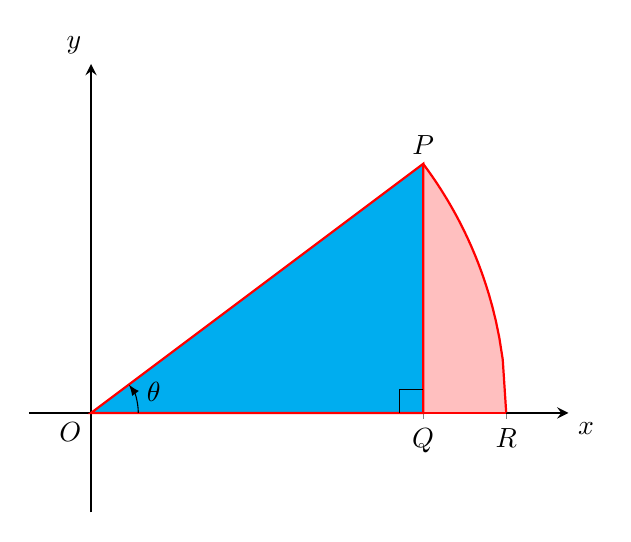
\begin{tikzpicture}[scale=1]
\begin{axis}[standard,xmin=0,trig format=deg,xtick={0.8,1},xticklabels={$Q$,$R$},ytick={\empty},xlabel={$x$},ylabel={$y$}]
\addplot[domain=0.8:1,red,thick,name path=F]{(1-x^2)^(1/2)};
\coordinate (A) at (0,0);
\coordinate (B) at (0.8,0.6);
\coordinate (C) at (0.8,0);
\draw[red,thick,fill=cyan] (A) -- (B) -- (C) -- cycle;
\draw pic["$\theta$",draw,-latex,angle eccentricity=1.4, angle radius=0.6cm]{angle=C--A--B};
\draw pic[draw,-,angle eccentricity=1.4, angle radius=0.3cm]{right angle=B--C--A};
\node[anchor=north east] at (0,0) {$O$};
\node[anchor=south] at (0.8,0.6) {$P$};
\draw[red,thick,name path=G] (0.8,0) -- (1,0);
\addplot[fill=pink] fill between [of=F and G, soft clip={domain=0.8:1}];
\end{axis}
\end{tikzpicture}

\[A=\frac{r^2}{2}\sin\theta\cos\theta+\int_{r\cos\theta}^r\sqrt{r^2-x^2}\ dx\]
\[\mbox{let }x=r\sin\theta,\ dx=r\cos\theta\ d\theta\]

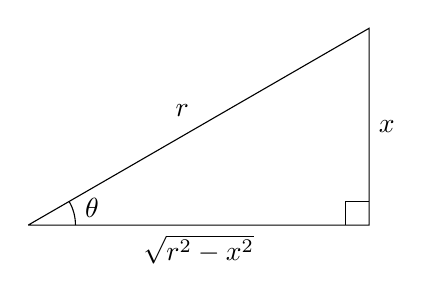
\begin{tikzpicture}[scale=5]
\coordinate (A) at (0,0);
\coordinate (B) at (30:1);
\coordinate (C) at (30:1|-0,0);
\draw (A) -- node[pos=0.5,above left]{$r$} (B) -- node[pos=0.5,right]{$x$} (C) -- node[pos=0.5,below]{$\sqrt{r^2-x^2}$} (A);
\draw pic["$\theta$",draw,-,angle eccentricity=1.4, angle radius=0.6cm]{angle=C--A--B};
\draw pic[draw,-,angle eccentricity=1.4, angle radius=0.3cm]{right angle=B--C--A};
\end{tikzpicture}

Now we will solve the indefinite integral $\int\sqrt{r^2-x^2}\ dx$.

\begin{align*}
\int\sqrt{r^2-x^2}&\overset{x=r\sin\theta}{\underset{dx=r\cos\theta\ d\theta}{=\joinrel=\joinrel=\joinrel=\joinrel=\joinrel=\joinrel=\joinrel=}}r^2\int\cos^2\theta\ d\theta\\
&=\frac{r^2}{2}\int1+\cos2\theta\ d\theta\\
&=\frac{r^2}{2}\left[\theta+\frac{1}{2}\sin2\theta\right]+C\\
&=\frac{r^2}{2}[\theta+\sin\theta\cos\theta]+C\\
&=\frac{r^2}{2}\left[\arcsin\frac{x}{r}+\frac{x}{r}\cdot\frac{\sqrt{r^2-x^2}}{r}\right]+C
\end{align*}

Now we will apply the original boundary conditions:

\begin{align*}
\frac{r^2}{2}\left[\arcsin\frac{x}{r}+\frac{x}{r}\cdot\frac{\sqrt{r^2-x^2}}{r}\right]_{r\cos\theta}^r&=\left[\frac{r^2}{2}\cdot\frac{\pi}{2}+0\right]-\left[\frac{r^2}{2}\cdot\arcsin(\cos\theta)+\frac{r^2}{2}\cos\theta\sin\theta\right]\\
&=\left[\frac{r^2}{2}\cdot\frac{\pi}{2}+0\right]-\left[\frac{r^2}{2}\left(\frac{\pi}{2}-\theta\right)+\frac{r^2}{2}\cos\theta\sin\theta\right]\\
&=\frac{r^2}{2}\theta-\frac{r^2}{2}\cos\theta\sin\theta
\end{align*}

Therefore,

\[\frac{r^2}{2}\sin\theta\cos\theta+\int_{r\cos\theta}^r\sqrt{r^2-x^2}\ dx=\frac{r^2}{2}\sin\theta\cos\theta+\frac{r^2}{2}\theta-\frac{r^2}{2}\cos\theta\sin\theta=\frac{r^2}{2}\theta\]

\end{document}